To map the regulatory system of WTO DSB with 
a network of legal articles of WTO agreement,
this paper introduces a novel design of deep neural network (Figure \ref{fig:traditional-convolutional-network}) that
gets two different types of input.
One is textual description of trade policy that led to the dispute and
the other one is the content of a legal article of the WTO agreement.
This design is improvised to mimic
the reasoning process of the legal practitioners
where the legal practitioners read
the text description of
factual circumstances of the dispute and think about the contents of
the applicable legal articles at the same time.
To train this neural network, I collected textual description of trade policy 
that led to the dispute and articles of the WTO agreement cited for each dispute
case requested to the WTO DSB 
from 1995 to 2018 (Table \ref{table: vardescription}).
Then I trained this neural network to answer correctly 
about whether the given article of the WTO agreement
can be cited for the given textual description of 
trade policy that led to the dispute.
After training, I collected all the answers of the trained neural network 
and created a network of legal articles of the WTO agreement (Figure \ref{fig:market-aceess_directed}) using 
the collected answers from the neural network (Figure \ref{predidction_matrix}).


% == THREE SUBSYSTEM == 
\begin{figure}
    \centering{
      \begin{tikzpicture}[>={Stealth[color=black]},shorten >=1pt,node distance=2cm,on grid,initial/.style={}]
  \node[state, label=right:Interpretation of Tariff Concession] (T1) {II:1};
  \node[state, label=left:General Elimination of Quantitative Restrictions] at ([shift=({240:3 cm})]T1) (T4) {XI:1};
  \node[state, label=right:Fair Adminstration of Laws and Regulations] at ([shift=({240:3 cm})]T4) (T5) {X:3(a)};
  \node[state, label=above:Non-discriminatory Administration of Quantitative Restrictions] at ([shift=({100:6 cm})]T4) (T7) {XIII:1};
  \node[state, label=right:National Treatment on Internal Taxation] at ([shift=({10:2.5 cm})]T4) (T6) {III:2};
  \node[state, label=above:Fees Connected with Importation and Exportation] at ([shift=({150:5.5 cm})]T4) (T8) {VIII};

  \begin{scope}[every edge/.append style={->, double=black, draw=white}] % for directed edge, change "style={->, double=black, draw=white}]"
    \path (T1)
    edge   (T4)
    edge   (T6);
    \path (T4)
    edge   (T5)
    edge   (T6)
    edge   (T7);
    \path (T5)
    edge   (T6);
    \path (T8)
    edge   (T7)
    edge   (T1)
    edge   (T6);

  \end{scope}
\end{tikzpicture}

% to draw the node's border w/ color, refer to https://tex.stackexchange.com/questions/438412/how-to-add-border-to-a-node
    }
    \caption{{\bf Network of the Articles of the WTO Agreement:} 
    This figure demonstrates a network of articles of WTO agreements
    that achieves \textit{Market Access} principle together.
    }
    \label{fig:market-aceess_directed}
  \end{figure}
  
\begin{figure}[t!]
	\centering
	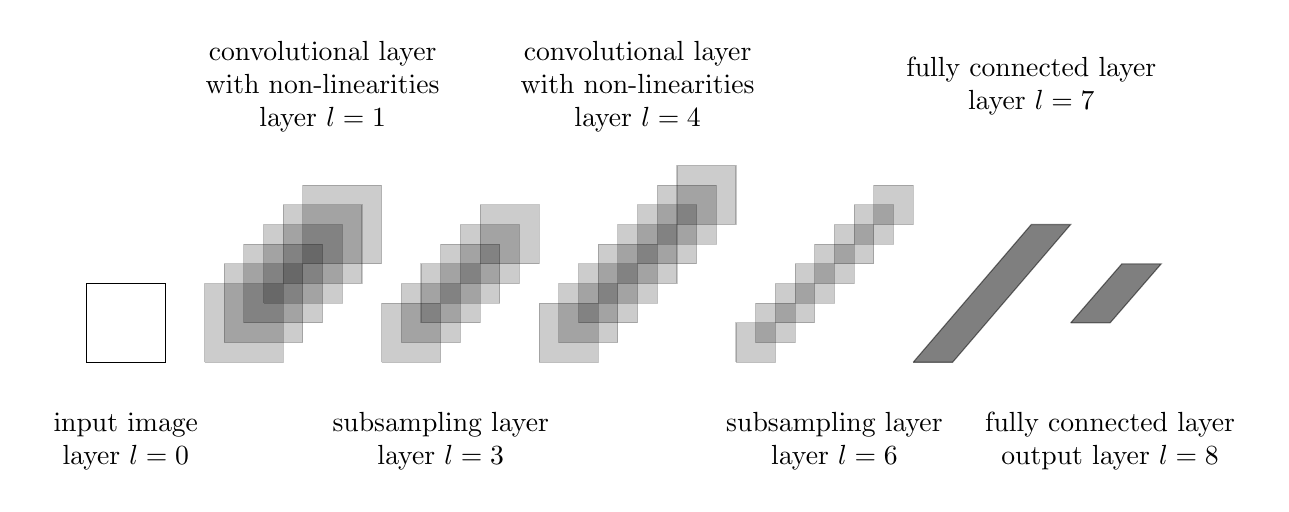
\begin{tikzpicture}
		\node at (0.5,-1){\begin{tabular}{c}input image\\layer $l = 0$\end{tabular}};
		
		\draw (0,0) -- (1,0) -- (1,1) -- (0,1) -- (0,0);
		
		\node at (3,3.5){\begin{tabular}{c}convolutional layer\\with non-linearities\\layer $l = 1$\end{tabular}};
		
		\draw[fill=black,opacity=0.2,draw=black] (2.75,1.25) -- (3.75,1.25) -- (3.75,2.25) -- (2.75,2.25) -- (2.75,1.25);
		\draw[fill=black,opacity=0.2,draw=black] (2.5,1) -- (3.5,1) -- (3.5,2) -- (2.5,2) -- (2.5,1);
		\draw[fill=black,opacity=0.2,draw=black] (2.25,0.75) -- (3.25,0.75) -- (3.25,1.75) -- (2.25,1.75) -- (2.25,0.75);
		\draw[fill=black,opacity=0.2,draw=black] (2,0.5) -- (3,0.5) -- (3,1.5) -- (2,1.5) -- (2,0.5);
		\draw[fill=black,opacity=0.2,draw=black] (1.75,0.25) -- (2.75,0.25) -- (2.75,1.25) -- (1.75,1.25) -- (1.75,0.25);
		\draw[fill=black,opacity=0.2,draw=black] (1.5,0) -- (2.5,0) -- (2.5,1) -- (1.5,1) -- (1.5,0);
		
		\node at (4.5,-1){\begin{tabular}{c}subsampling layer\\layer $l = 3$\end{tabular}};
		
		\draw[fill=black,opacity=0.2,draw=black] (5,1.25) -- (5.75,1.25) -- (5.75,2) -- (5,2) -- (5,1.25);
		\draw[fill=black,opacity=0.2,draw=black] (4.75,1) -- (5.5,1) -- (5.5,1.75) -- (4.75,1.75) -- (4.75,1);
		\draw[fill=black,opacity=0.2,draw=black] (4.5,0.75) -- (5.25,0.75) -- (5.25,1.5) -- (4.5,1.5) -- (4.5,0.75);
		\draw[fill=black,opacity=0.2,draw=black] (4.25,0.5) -- (5,0.5) -- (5,1.25) -- (4.25,1.25) -- (4.25,0.5);
		\draw[fill=black,opacity=0.2,draw=black] (4,0.25) -- (4.75,0.25) -- (4.75,1) -- (4,1) -- (4,0.25);
		\draw[fill=black,opacity=0.2,draw=black] (3.75,0) -- (4.5,0) -- (4.5,0.75) -- (3.75,0.75) -- (3.75,0);
		
		\node at (7,3.5){\begin{tabular}{c}convolutional layer\\with non-linearities\\layer $l = 4$\end{tabular}};
		
		\draw[fill=black,opacity=0.2,draw=black] (7.5,1.75) -- (8.25,1.75) -- (8.25,2.5) -- (7.5,2.5) -- (7.5,1.75);
		\draw[fill=black,opacity=0.2,draw=black] (7.25,1.5) -- (8,1.5) -- (8,2.25) -- (7.25,2.25) -- (7.25,1.5);
		\draw[fill=black,opacity=0.2,draw=black] (7,1.25) -- (7.75,1.25) -- (7.75,2) -- (7,2) -- (7,1.25);
		\draw[fill=black,opacity=0.2,draw=black] (6.75,1) -- (7.5,1) -- (7.5,1.75) -- (6.75,1.75) -- (6.75,1);
		\draw[fill=black,opacity=0.2,draw=black] (6.5,0.75) -- (7.25,0.75) -- (7.25,1.5) -- (6.5,1.5) -- (6.5,0.75);
		\draw[fill=black,opacity=0.2,draw=black] (6.25,0.5) -- (7,0.5) -- (7,1.25) -- (6.25,1.25) -- (6.25,0.5);
		\draw[fill=black,opacity=0.2,draw=black] (6,0.25) -- (6.75,0.25) -- (6.75,1) -- (6,1) -- (6,0.25);
		\draw[fill=black,opacity=0.2,draw=black] (5.75,0) -- (6.5,0) -- (6.5,0.75) -- (5.75,0.75) -- (5.75,0);
		
		\node at (9.5,-1){\begin{tabular}{c}subsampling layer\\layer $l = 6$\end{tabular}};
		
		\draw[fill=black,opacity=0.2,draw=black] (10,1.75) -- (10.5,1.75) -- (10.5,2.25) -- (10,2.25) -- (10,1.75);
		\draw[fill=black,opacity=0.2,draw=black] (9.75,1.5) -- (10.25,1.5) -- (10.25,2) -- (9.75,2) -- (9.75,1.5);
		\draw[fill=black,opacity=0.2,draw=black] (9.5,1.25) -- (10,1.25) -- (10,1.75) -- (9.5,1.75) -- (9.5,1.25);
		\draw[fill=black,opacity=0.2,draw=black] (9.25,1) -- (9.75,1) -- (9.75,1.5) -- (9.25,1.5) -- (9.25,1);
		\draw[fill=black,opacity=0.2,draw=black] (9,0.75) -- (9.5,0.75) -- (9.5,1.25) -- (9,1.25) -- (9,0.75);
		\draw[fill=black,opacity=0.2,draw=black] (8.75,0.5) -- (9.25,0.5) -- (9.25,1) -- (8.75,1) -- (8.75,0.5);
		\draw[fill=black,opacity=0.2,draw=black] (8.5,0.25) -- (9,0.25) -- (9,0.75) -- (8.5,0.75) -- (8.5,0.25);
		\draw[fill=black,opacity=0.2,draw=black] (8.25,0) -- (8.75,0) -- (8.75,0.5) -- (8.25,0.5) -- (8.25,0);
		
		\node at (12,3.5){\begin{tabular}{c}fully connected layer\\layer $l = 7$\end{tabular}};
		
		\draw[fill=black,draw=black,opacity=0.5] (10.5,0) -- (11,0) -- (12.5,1.75) -- (12,1.75) -- (10.5,0);
		
		\node at (13,-1){\begin{tabular}{c}fully connected layer\\output layer $l = 8$\end{tabular}};
		
		\draw[fill=black,draw=black,opacity=0.5] (12.5,0.5) -- (13,0.5) -- (13.65,1.25) -- (13.15,1.25) -- (12.5,0.5);
	\end{tikzpicture}
	\caption[Architecture of a traditional convolutional neural network.]{The architecture of the original convolutional neural network, as introduced by LeCun et al. (1989).}
	\label{fig:traditional-convolutional-network}
\end{figure}
 


\begin{xltabular}{\linewidth}{ l | X }
    \caption{Description of Variables used in this Study} 
   \label{table: vardescription}\\
   \hline \hline
  
  \textbf{\normalsize Code} & \textbf{\normalsize Definition and source \Checkmark}  \\
   \hline 
  \endfirsthead
   \hline \hline
  
  \textbf{\normalsize Code} & \textbf{\normalsize Definition and source}  \\
   \hline 
  \endhead
  
  \textbf{exportsgr} & Exports of goods and services (annual \% growth) retrieved from World Bank. \\ \hline 
  
  
  \textbf{importsgr} & Imports of goods and services (annual \% growth) retrieved from World Bank.\\ \hline 
  
  
  \textbf{gr\_tot} & Terms of trade change over previous year (in \%).  Data for terms of trade are collected from theglobaleconomy.com  and Kaminsky and Reinhart online database. Since variables have two different base years, the base year for both was changed to 2000 to have the same base year. And then the change is calculated as below.  
  
  \begin{equation}
  gr\_tot_{i,t} = (\frac{tot_{i,t}- tot_{i,t-1}}{tot_{i,t-1}})100
  \end{equation}
  \\ \hline
  
  \end{xltabular}



% where nodes are the articles of the WTO agreement and the edges are ranking of importance between incoming nodes to each 
% target node using a tree-based ensemble machine learning method 
% using the answers of the trained neural network.
%, called GENIE3 \citep{genie3} 
